\part{Capítulo doce}

%----------------------------------------------------------------------------------------
%	CHAPTER 12
%----------------------------------------------------------------------------------------
\graphicspath{ {12_Capitulo/img/ejemplos/}, {W_Varios/2_Portada_capitulos/} }

\chapterimage{ima2} % Chapter heading image


\chapter{Relación Beneficio/Costo}

\section{Mapa Mental}

\begin{center}
   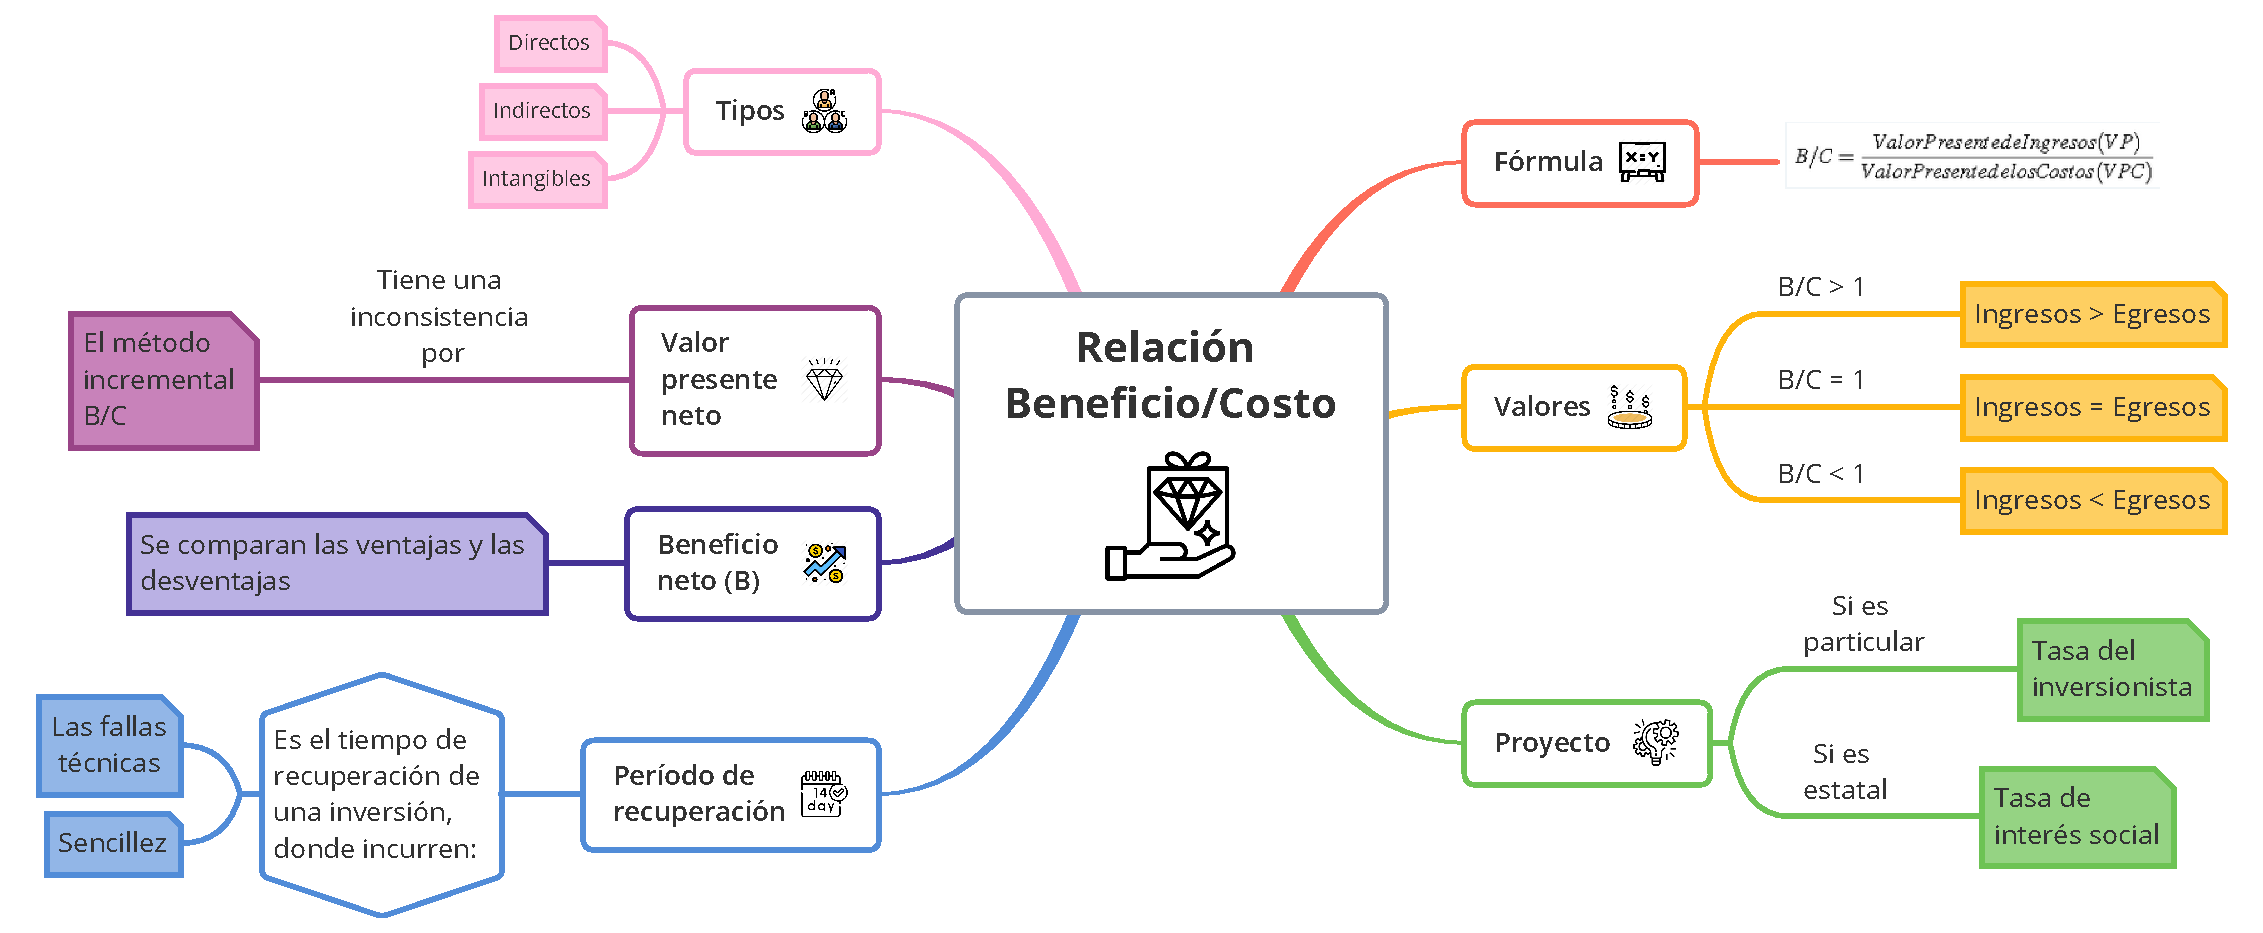
\includegraphics[height=6cm]{Mapa Mental 12.1.pdf}
\end{center} 


\section{Formulas de los capítulos}

\begin{spacing}{1.5}
	\begin{center}
		\begin{tabular}{ |p{4cm}|p{7cm}| p{4cm}|}
			\hline
			\rowcolor{orange!50}
			\begin{center}\textbf{Fórmula} \end{center} & \begin{center} \textbf{Nombre}\end{center}             & \begin{center} \textbf{Excel} \end{center}             \\ \hline
			
			B/C = $\frac{VPN}{VPC}$   & Relación Beneficio/Costo              & B/C = beneficio / (costo + Inversión) \\ \hline
			
			VP = $\frac{R}{i}$        & Valor Presente Serie Perpetua Vencida &                                       \\ \hline
		\end{tabular}
	\end{center}
\end{spacing}

\section{Introducción}
La relación Beneficio/Costo (B/C), consiste en poner en valor presente los beneficios netos y dividirlos por el valor presente de todos los costos del proyecto. La tasa que se utilice para poner en valor presente, tanto los beneficios como los costos, depende de quien lleve a cabo el proyecto, si el proyecto es particular se utiliza la tasa del inversionista, pero si éste es estatal se puede usar la tasa de interés social (que es más baja lo cual hace que la aceptación sea mas probable), de acuerdo a lo anterior podemos plantear la siguiente ecuación:

\begin{equation}
	B/C = \frac{Valor Presente de Ingresos(VP)}{Valor Presente de Costos(VPC)} \hspace{35pt} \textit{Relación Beneficio Costo (B/C)}
\end{equation}

La Relación B/C puede por tanto tomar tres valores:

% Incluir grafica 12_1
\begin{center}
	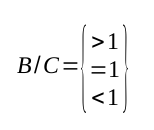
\includegraphics[height=3.0cm]{E12_1}
\end{center}

Si B/C < 1 significa que los ingresos son menores que los costos, por tanto el proyecto no es aconsejable.
\\
Si B/C = 1 significa que un valor presente, los ingresos son iguales a los egresos, en éste caso, lo único que se alcanza a ganar es la tasa del inversionista, por lo tanto es indiferente realizar el proyecto o continuar con la inversión que normalmente hace el inversionista.
\\
Si B/C  > 1 significa que en valor presente, los ingresos son mayores que los egresos, por lo tanto se aconseja realizar el proyecto.
\\
Las entidades crediticias tales como: Banco Mundial, Banco Internacional de Desarrollo, Fondo Monetario Internacional, etc., acostumbran a evaluar sus proyectos de inversión mediante la Relación B/C y adicionalmente con otro índice que generalmente es el VPN(Valor Presente Neto). Por esto es de gran importancia que cualquier proyecto que debido a su tamaño necesite financiación internacional sea evaluado con la Relación B/C.

\section{Beneficios, déficit , ventajas y desventajas en los proyectos}

Por lo general, los grandes proyectos son propiedad del estado y producen un beneficio para la sociedad,pero a su vez también pueden causar perdidas a las que llamaremos déficit  o desventajas y los costos del proyecto son los dineros invertidos por el estado.
\\
Es importante aclarar que el beneficio neto se representara con la letra B, es decir el beneficio menos el déficit. Para facilitar la identificación de las cantidades que corresponden a beneficios, déficit  y costos, podemos asumir, que en proyectos estatales, el que recibe los beneficios es la sociedad, el que recibe los déficit  también es la sociedad y el que hace los gastos es el estado. En proyectos particulares, el dueño del proyecto es quién recibe los beneficios, los déficit  y a su vez es el que hace sus gastos.
\\

%%%%%%%%%%% NO OLVIDAR COLOCAR ESTE COMENTARIO CON EL NUMERO DE EJERCICIO %%%%%%%%%%%%%
%%%%%%%%%%%%%%%%%%%% EJERCICIO 1 %%%%%%
%%%Text bf para negrilla , el \\ es para el salto de linea.
%%%El primer \\ hace un espacio en el texto y el 2 \\ crea otro espacio
%\begin{minipage}{\textwidth}
%	\textbf{Ejemplo 1}\newline
%	¿A qué tasa periódica mes vencida,  COP 30{.}000 se convertirán en  COP 35{.}000 en 6 meses?\\ \\
%	\textbf{Solución.}\\
%	\begin{center}
%
%		\renewcommand{\arraystretch}{1.5}% Margenes de las celdas
%		%Creación de la cuadricula
%		\begin{tabular}{|c|c|c| }
%			%Creamos una linea horizontal
%			\hline
%			%Definimos el color de la primera fila
%			\rowcolor[HTML]{FFB183}
%			%%%%% INICIO ASIGNACIÓN FECHA FOCAL %%%%%%%
%			%%%%%%%%%% INICIO TITULO
%			%Lo que se hace aquí es mezclar las 3 columnas en una sola
%			\multicolumn{3}{|c|}{\cellcolor[HTML]{FFB183}\textbf{1. Asignación período focal}}   \\ \hline
%			%%%%%%%%%% FIN TITULO
%			%%%%% INICIO DECLARACIÓN DE VARIABLES %%%%%%%
%			\multicolumn{3}{|c|}{$pf = 6pmv$} \\ \hline
%			%Definimos el color de la primera fila
%			\rowcolor[HTML]{FFB183}
%			%%%%% INICIO DECLARACIÓN DE VARIABLES %%%%%%%
%			%%%%%%%%%% INICIO TITULO
%			\multicolumn{3}{|c|}{\cellcolor[HTML]{FFB183}\textbf{2. Declaración de variables}}                                                                                   \\ \hline
%			%%%%%%%%%% FIN TITULO
%			%%%%%%%%%% INICIO DE MATEMÁTICAS
%			$F =  COP 35\,000$                                                       & $n = 6 \textit{  pmv}$                                                       & $i =  COP ? pmv$ \\
%			$P =  COP 30\,000$                                                       &                                                                              &               \\ \hline
%			%%%%%%%%%% FIN DE MATEMÁTICAS
%			%%%%% FIN DECLARACIÓN DE VARIABLES
%			
%			
%			%%%%% INICIO FLUJO DE CAJA
%			\rowcolor[HTML]{FFB183}
%			\multicolumn{3}{|c|}{\cellcolor[HTML]{FFB183}\textbf{3. Diagrama de flujo de caja}}                                                                                  \\ \hline
%			%Mezclamos 3 columnas y pondremos el dibujo
%			%%%%%%%%%%%%% INSERCIÓN DE LA IMAGEN
%			\multicolumn{3}{|c|}{ 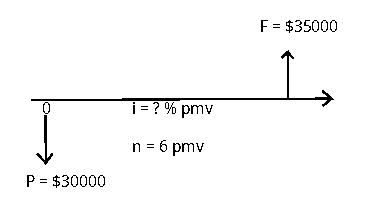
\includegraphics[scale=1.2]{1/capitulo1ejemplo1.pdf} }                                                                                         \\ \hline
%			%%%%%%%%%%%%% FIN INSERCIÓN DE IMAGEN
%			%%%%%FIN FLUJO DE CAJA
%			
%			
%			
%			%%%%% INICIO DECLARACIÓN FORMULAS
%			%%%%%%%%%%% INICIO TITULO
%			\rowcolor[HTML]{FFB183}
%			\multicolumn{3}{|c|}{\cellcolor[HTML]{FFB183}\textbf{4. Declaración de fórmulas}}                                                                                    \\ \hline
%			%%%%%%%%%%% FIN TITULO
%			%%%%%%%%%%% INICIO MATEMÁTICAS
%			
%			$F = P(1+in) \hspace{0.3cm} \textit{Valor futuro}$                   & \multicolumn{2}{c|}{$i = \frac{F}{nP}-\frac{1}{n} \hspace{0.3cm}\textit{Tasa de interés periódica}$}                      \\ \hline
%			%%%%%%%%%% FIN MATEMÁTICAS
%			%%%%%% INICIO DESARROLLO MATEMÁTICO
%			\rowcolor[HTML]{FFB183}
%			%%%%%%%%%%INICIO TITULO
%			\multicolumn{3}{|c|}{\cellcolor[HTML]{FFB183}\textbf{5. Desarrollo matemático}}                                                                                      \\ \hline
%			%%%%%%%%%% FIN TITULO
%			%%%%%%%%%% INICIO MATEMÁTICAS
%			 \multicolumn{3}{|c|}{$i =\frac{ COP 35{.}000}{6\cdot  COP 30{.}000}-\frac{1}{6}=0.2778$}                 \\ \hline
%			%%%%%%%%%% FIN MATEMÁTICAS
%			%%%%%% FIN DESARROLLO MATEMÁTICO
%			
%			\rowcolor[HTML]{FFB183}
%			\multicolumn{3}{|c|}{\cellcolor[HTML]{FFB183}\textbf{6. Respuesta}}    \\ \hline    
%			
%			\multicolumn{3}{|c|}{$i = 2.778\%pmv$} \\ \hline
%		\end{tabular}
%		%Se crean dos lineas en blanco para que no quede el siguiente texto tan pegado
%		\newline \newline
%	\end{center}
%\end{minipage}
%%%%%%%%%%%%%%%%%%%%%%%%%%%FIN EJERCICIO X %%%%%%%%%%%%%%%%%%%%%%%%%%%



\section{Relación B/C Y VPN}
Ocasionalmente se puede presentar una inconsistencia cuando se evalúan alternativas con la Relación B/C y con el VPN, en tales circunstancias el error debe estar en la Relación B/C causado por un incorrecto cálculo de los beneficios, entonces, se debe analizar lo que pasa con el exceso de inversión, es decir, que debe aplicarse el método incremental en la Relación B/C.
\\

%%%%%%%%%% NO OLVIDAR COLOCAR ESTE COMENTARIO CON EL NUMERO DE EJERCICIO %%%%%%%%%%%%%
%%%%%%%%%%%%%%%%%%% EJERCICIO 2 %%%%%%
%%Text bf para negrilla , el \\ es para el salto de linea.
%%El primer \\ hace un espacio en el texto y el 2 \\ crea otro espacio
\textbf{Ejemplo 2}\newline
El jefe de producción de una fábrica debe decidir entre dos máquinas A y B. Las características de cada una son: \\
\begin{center}
		\begin{tabular}{|p{1cm}|p{2cm}|p{2cm}|p{2cm}|p{3cm}|}
			\hline
			\rowcolor{white!50}
			\textbf{Maq.} & \textbf{C} & \textbf{K} & \textbf{S} & \textbf{CAO} \\ \hline
			A            & 800.000 COP   & 3 años     & 200.000 COP    & 25.000 COP       \\ \hline
			B            & 600.000 COP   & 2 años     & 150.000 COP    & 30.000 COP       \\ \hline
		\end{tabular}
\end{center}

Con una tasa del 36\% nominal anual año vencido, determinar la mejor alternativa.

\textbf{Solución.}\\
\begin{center}
	\renewcommand{\arraystretch}{1.5}% Margenes de las celdas
	%Creación de la cuadricula
	\begin{longtable}[H]{|c|c|c|}
		%Creamos una linea horizontal
		\hline
		%Definimos el color de la primera fila
		\rowcolor[HTML]{FFB183}
		%%%%% INICIO ASIGNACIÓN FECHA FOCAL %%%%%%%
		%%%%%%%%%% INICIO TITULO
		%Lo que se hace aquí es mezclar las 3 columnas en una sola
		\multicolumn{3}{|c|}{\cellcolor[HTML]{FFB183}\textbf{1. Asignación período focal}}   \\ \hline
		%%%%%%%%%% FIN TITULO
		%%%%% INICIO DECLARACIÓN DE VARIABLES %%%%%%%
		\multicolumn{3}{|c|}{$pf = 0  \textit{ pav }$} \\ \hline
		%Definimos el color de la primera fila
		\rowcolor[HTML]{FFB183}
		%%%%% INICIO DECLARACIÓN DE VARIABLES %%%%%%%
		%%%%%%%%%% INICIO TITULO
		\multicolumn{3}{|c|}{\cellcolor[HTML]{FFB183}\textbf{2. Declaración de variables}}                                                                                   \\ \hline
		%%%%%%%%%% FIN TITULO
		%%%%%%%%%% INICIO DE MATEMÁTICAS
		$\text{Alternativa A}$ & $\text{Alternativa B}$ & $i= 36\% \text{ pav }$\\
		$C =  800{.}000\text{ COP}$ & $C =  600{.}000\text{ COP}$ & $CPUE =  ?\text{ COP}$\\
		$K =  3 \textit{ años}$ & $K =  2 \textit{ años}$ & \\
		$S =  200{.}000\text{ COP}$ & $S =  150{.}000\text{ COP}$ & \\
		$CAO =  25{.}000\text{ COP}$ & $CAO =  30{.}000\text{ COP}$ & \\
 		$n_{1}= 3 \text{ pav}$ & $n_{2}= 2 \text{ pav}$ &   \\\hline 
		%%%%%%%%%% FIN DE MATEMÁTICAS
		%%%%% FIN DECLARACIÓN DE VARIABLES


		%%%%% INICIO FLUJO DE CAJA
		\rowcolor[HTML]{FFB183}
		\multicolumn{3}{|c|}{\cellcolor[HTML]{FFB183}\textbf{3. Diagrama de flujo de caja}}\\ \hline
		%Mezclamos 3 columnas y pondremos el dibujo
		%%%%%%%%%%%%% INSERCIÓN DE LA IMAGEN
		\multicolumn{3}{|c|}{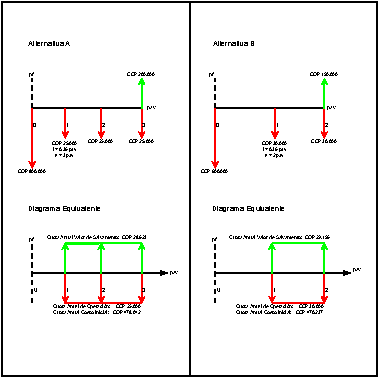
\includegraphics[trim=-5 -5 -5 -5 , scale=2]{10_Capitulo/ejemplos/2/Ejemplo_2.pdf}}
        \\\hline
		%%%%%%%%%%%%% FIN INSERCIÓN DE IMAGEN
		%%%%%FIN FLUJO DE CAJA



		%%%%% INICIO DECLARACIÓN FORMULAS
		%%%%%%%%%%% INICIO TITULO
		\rowcolor[HTML]{FFB183}
		\multicolumn{3}{|c|}{\cellcolor[HTML]{FFB183}\textbf{4. Declaración de fórmulas}} \\ \hline
		%%%%%%%%%%% FIN TITULO
		%%%%%%%%%%% INICIO MATEMÁTICAS

		\multicolumn{3}{|c|}{$VP=R\frac{1-(1+i_{1})^{-n}}{i_{2}} \text{ Valor presente serie uniforme vencida}$}\\ 
		\multicolumn{3}{|c|}{$VF=R\frac{1-(1+i_{1})^{n}}{i_{2}} \text{ Valor futuro aserie uniforme vencida}$}\\\hline
		%%%%%%%%%% FIN MATEMÁTICAS
		%%%%%% INICIO DESARROLLO MATEMÁTICO
		\rowcolor[HTML]{FFB183}
		%%%%%%%%%%INICIO TITULO
		\multicolumn{3}{|c|}{\cellcolor[HTML]{FFB183}\textbf{5. Desarrollo matemático}}   \\ \hline
		%%%%%%%%%% FIN TITULO
		%%%%%%%%%% INICIO MATEMÁTICAS
		Alternativa A & \multicolumn{2}{c|}{Alternativa B}\\ \hline
		Cuota anual costo inicial & \multicolumn{2}{c|}{Cuota anual costo inicial} \\
		${R=\frac{800{.}000}{\frac{1-(1,36)^{-3}}{0,36}} = 178{.}042}\text{ COP}$ & \multicolumn{2}{c|}{${R=\frac{600{.}000}{\frac{1-(1,36)^{-2}}{0,36}} = 470{.}237 }\text{ COP}$} \\
		Cuota anual valor salvamento & \multicolumn{2}{c|}{Cuota anual valor salvamento}\\
		$R=\frac{200{.}000}{\frac{(1,36)^{3}}{0,36}} = 28{.}623\text{ COP} $ & \multicolumn{2}{c|}{$R=\frac{150{.}000}{\frac{(1,36)^{2}}{0,36}} = 29{.}196 \text{ COP}$} \\
		CPUE alternativa A & \multicolumn{2}{c|}{CPUE alternativa B} \\ 
		$CPUE_{A} = 28.623-478.042-25.000 $ & \multicolumn{2}{c|}{$CPUE_{B} = 29.196-470.237-30.000$}\\ 
		$CPUE_{A} = -474.419\text{ COP}$ & \multicolumn{2}{c|}{$CPUE_{B} = -471.04$\text{ COP}}\\
		\hline
		%%%%%%%%%% FIN MATEMÁTICAS
		%%%%%% FIN DESARROLLO MATEMÁTICO

		\rowcolor[HTML]{FFB183}
		\multicolumn{3}{|c|}{\cellcolor[HTML]{FFB183}\textbf{6. Respuesta}}    \\ \hline

		\multicolumn{3}{|c|}{La alternativa que representa menores perdidad es la B.} \\ 
		\hline
	\end{longtable}
	%Se crean dos lineas en blanco para que no quede el siguiente texto tan pegado
	%\newline \newline
\end{center}
%%%%%%%%%%%%%%%%%%%%%%%%%%FIN EJERCICIO X %%%%%%%%%%%%%%%%%%%%%%%%%%%





\section{Periodo de recuperación}
El Período de Recuperación, PR, es otro índice utilizado para medir la bondad de un proyecto, sin embargo este ha venido perdiendo popularidad dandole paso al VPN y a la TIR que son mucho más exactos. El PR es el tiempo que debe utilizarse para recuperar la inversión, sin tener en cuenta los intereses; Por ejemplo, si se invierten  COP 600.000 en un proyecto que produce  COP 200.000 anuales durante 8 años, entonces se necesitarán 3 años para recuperar la inversión inicial (3 x 200.000 = 600.000) y, de ahí en adelante, lo que se produzca se considera ganancia. Si el propietario del proyecto considera que 3 años es un tiempo razonable para recuperar la inversión, el proyecto será aceptado, pero si considera que no puede esperar tanto tiempo, el proyecto será rechazado.\\

Entre las fallas técnicas que presenta el PR está la de no tomar en cuenta el valor del dinero a través del tiempo y la de no tomar en cuenta el flujo de caja después de la recuperación de los dineros invertidos. En el siguiente ejemplo, se podrán observar estas fallas.\\

\textbf{Ejemplo 3}\\
Hallar el valor presente de la siguiente serie con una tasa del 5\% periodo anual mes vencido, utilizando dos formas para resolverlo.\\

%imagen 4
\begin{center}
	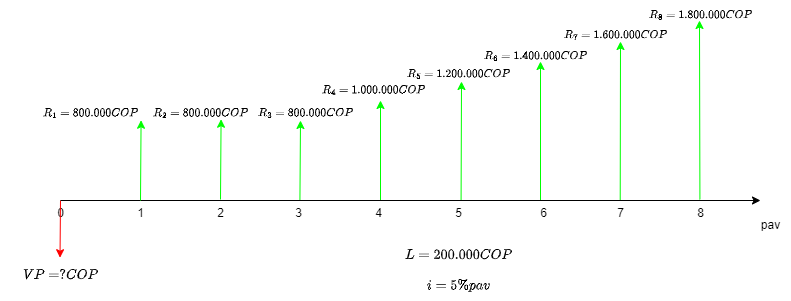
\includegraphics[height=4.0cm]{6_Capitulo/img/ejemplos/6_5}
\end{center}

\textbf{Solución:}

\begin{center}
	\textbf{Primera forma:}
\end{center}

%La tabla ira centrada
\begin{center}
	\renewcommand{\arraystretch}{1.4}% Margenes de las celdas
	%Creación de la cuadricula de 3 columnas
	\begin{longtable}[H]{|c|c|c|}
		%Creamos una linea horizontal
		\hline
		%Definimos el color de la primera fila
		\rowcolor[HTML]{FFB183}
		%%%%% INICIO ASIGNACIÓN PERIODO FOCAL %%%%%%%
		%%%%%%%%%% INICIO TITULO
		%Lo que se hace aquí es mezclar las 3 columnas en una sola
		\multicolumn{3}{|c|}{\cellcolor[HTML]{FFB183}\textbf{1. Asignación período focal}}                                                                                                                            \\ \hline
		\multicolumn{3}{|c|}{$Pf=0 \textit{ pav}$}                                                                                                                                                                    \\ \hline
		%%%%%%%%%% FIN TITULO
		%%%%% INICIO DECLARACIÓN DE VARIABLES %%%%%%%
		%%%%%%%%%% INICIO TITULO
		%Lo que se hace aquí es mezclar las 3 columnas en una sola
		\multicolumn{3}{|c|}{\cellcolor[HTML]{FFB183}\textbf{2. Declaración de variables}}                                                                                                                            \\ \hline
		%%%%%%%%%% FIN TITULO
		%%%%%%%%%% INICIO DE MATEMÁTICAS
		%Cada & hace referencia al paso de la siguiente columna
		\multicolumn{2}{|c|}{$\hspace{2 cm}R=800{.}000 COP \hspace{2 cm}$} & $i=5\%\textit{ pav}$                                                                                                                     \\
		\multicolumn{2}{|c|}{$L=  200{.}000COP$}                           & $n_1=2\textit{ pav}$                                                                                                                     \\
		\multicolumn{2}{|c|}{$VP= ?COP $}                                  & $n_2=6\textit{ pav}$                                                                                                                     \\\hline

		%%%%%%%%%% FIN DE MATEMÁTICAS
		%%%%% FIN DECLARACIÓN DE VARIABLES


		%%%%% INICIO FLUJO DE CAJA
		\rowcolor[HTML]{FFB183}
		\multicolumn{3}{|c|}{\cellcolor[HTML]{FFB183}\textbf{3. Diagrama de flujo de caja}}                                                                                                                           \\ \hline
		%Mezclamos 3 columnas y pondremos el dibujo
		%%%%%%%%%%%%% INSERCIÓN DE LA IMAGEN
		%Deberán descargar las imágenes respectivas del drive y pegarlas en la carpeta
		%n_capitulo/img/ejemplos/1/capitulo1ejemplo1.pdf  (el /1/ es el numero del ejemplo)
		\multicolumn{3}{|c|}{ 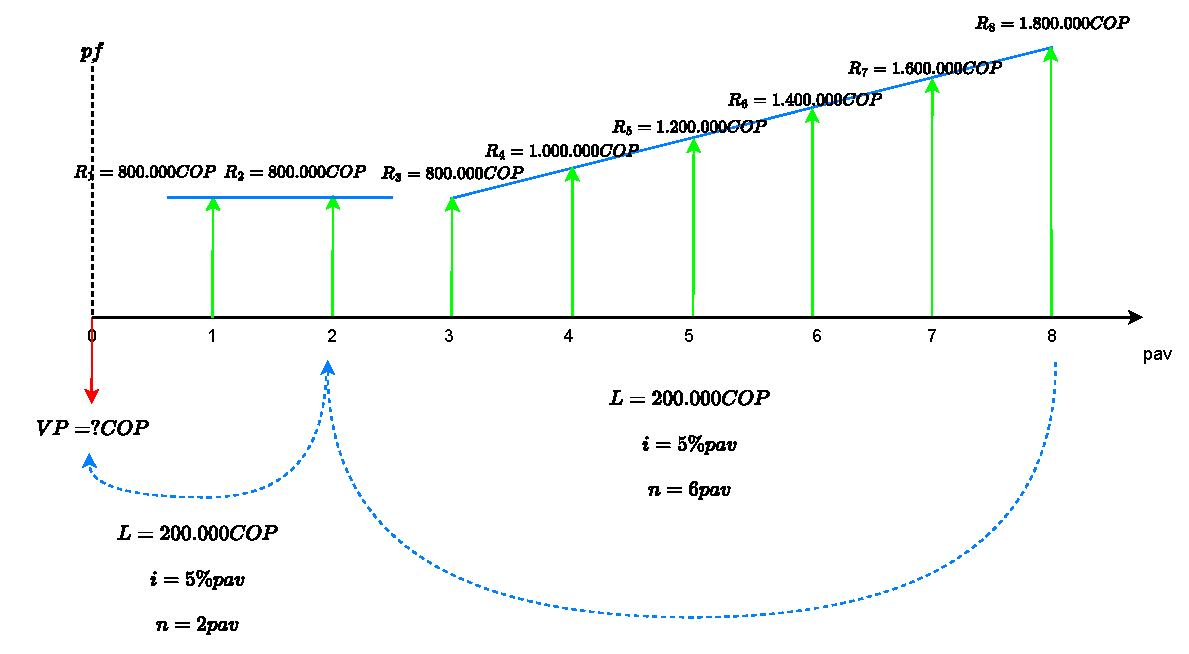
\includegraphics[trim=-5 -5 -5 -5 , scale=0.4]{6_Capitulo/ejemplos/3/Capitulo6Ejemplo3a.pdf} }

		\\ \hline
		%%%%%%%%%%%%% FIN INSERCIÓN DE IMAGEN
		%%%%%FIN FLUJO DE CAJA

		%%%%% INICIO DECLARACIÓN FORMULAS
		%%%%%%%%%%% INICIO TITULO
		\rowcolor[HTML]{FFB183}
		\multicolumn{3}{|c|}{\cellcolor[HTML]{FFB183}\textbf{4. Declaración de fórmulas}}                                                                                                                             \\ \hline
		%%%%%%%%%%% FIN TITULO
		%%%%%%%%%%% INICIO MATEMÁTICAS

		\multicolumn{3}{|c|}{$VP=R(\frac{1-(1+i)^{-n}}{i})+\frac{L}{i}[\frac{1-(1+i)^{-n}}{i}-n(1+i)^{-n}] \hspace{0.4 cm} \textit{Valor presente gradiente aritmético}$}                                             \\
		\multicolumn{3}{|c|}{$VP=R(\frac{1-(1+i)^{-n}}{i}) \hspace{0.4 cm} \textit{Valor presente de una serie unifrome vencida}$}                                                                                    \\
		\multicolumn{3}{|c|}{$P=F(1+i)^{-n} \hspace{0.4 cm} \textit{Valor presente dado un valor futuro}$}                                                                                                            \\ \hline

		%%%%%%%%%% FIN MATEMÁTICAS
		%%%%%% INICIO DESARROLLO MATEMÁTICO
		\rowcolor[HTML]{FFB183}
		%%%%%%%%%%INICIO TITULO
		\multicolumn{3}{|c|}{\cellcolor[HTML]{FFB183}\textbf{5. Desarrollo matemático}}                                                                                                                               \\ \hline
		%%%%%%%%%% FIN TITULO
		%%%%%%%%%% INICIO MATEMÁTICAS
		\multicolumn{3}{|c|}{$VP=  800{.}000COP(\frac{1-(1+0.05)^{-2}}{0.05})+[  800{.}000COP(\frac{1-(1+0.05)^{-6}}{0.05})+\frac{ COP 200{.}000}{0.05}[\frac{1-(1+0.05)^{-6}}{0.05}-6(1+0.05)^{-6}]]$} \\
		\multicolumn{3}{|c|}{$*(1+0.05)^{-2}$}\\
		\multicolumn{3}{|c|}{$VP= 7{.}341{.} \textit{  COP }$}                                                                                                                                                       \\ \hline


		%%%%%%%%%% FIN MATEMÁTICAS
		%%%%%% FIN DESARROLLO MATEMÁTICO
		%%%%%% INICIO RESPUESTA
		\rowcolor[HTML]{FFB183}
		%%%%%%%%%%INICIO TITULO
		\multicolumn{3}{|c|}{\cellcolor[HTML]{FFB183}\textbf{6. Respuesta}}                                                                                                                                           \\ \hline
		%%%%%%%%%% FIN TITULO
		%%%%%%%%%% INICIO RESPUESTA MATEMÁTICA
		\multicolumn{3}{|c|}{\textbf{$\textit{VP= 7{.}341{.}634.83  COP }$}}
		\\ \hline
		%%%%%%%%%% FIN MATEMÁTICAS
		%%%%%% FIN RESPUESTA
	\end{longtable}
	%Se crean dos lineas en blanco para que no quede el siguiente texto tan pegado
	%\newline \newline %USARLO SI CREES QUE ES NECESARIO
\end{center}
%%%%%%%%%%%%%%%%%%%%%%%%%%FIN EJERCICIO 3.1 %%%%%%%%%%%%%%%%%%%%%%%%%%%

\textbf{Segunda forma:}


%La tabla ira centrada
\begin{center}
	\renewcommand{\arraystretch}{1.4}% Margenes de las celdas
	%Creación de la cuadricula de 3 columnas
	\begin{longtable}[H]{|c|c|c|}
		%Creamos una linea horizontal
		\hline
		%Definimos el color de la primera fila
		\rowcolor[HTML]{FFB183}
		%%%%% INICIO ASIGNACIÓN PERIODO FOCAL %%%%%%%
		%%%%%%%%%% INICIO TITULO
		%Lo que se hace aquí es mezclar las 3 columnas en una sola
		\multicolumn{3}{|c|}{\cellcolor[HTML]{FFB183}\textbf{1. Asignación período focal}}                                                                                                                                                            \\ \hline
		\multicolumn{3}{|c|}{$pf=0 \textit{ pav}$}                                                                                                                                                                                                    \\ \hline
		%%%%%%%%%% FIN TITULO
		%%%%% INICIO DECLARACIÓN DE VARIABLES %%%%%%%
		%%%%%%%%%% INICIO TITULO
		%Lo que se hace aquí es mezclar las 3 columnas en una sola
		\multicolumn{3}{|c|}{\cellcolor[HTML]{FFB183}\textbf{2. Declaración de variables}}                                                                                                                                                            \\ \hline
		%%%%%%%%%% FIN TITULO
		%%%%%%%%%% INICIO DE MATEMÁTICAS
		%Cada & hace referencia al paso de la siguiente columna
		\multicolumn{2}{|c|}{$\hspace{2 cm}R=  800{.}000COP\hspace{2 cm}$} & $i=5\%\textit{ pav}$                                                                                                                                                     \\
		\multicolumn{2}{|c|}{$L=  200{.}000COP$}                           & $n_1=3\textit{ pav}$                                                                                                                                                     \\
		\multicolumn{2}{|c|}{$VP=? COP $}                                  & $n_2=5\textit{ pav}$                                                                                                                                                     \\\hline

		%%%%%%%%%% FIN DE MATEMÁTICAS
		%%%%% FIN DECLARACIÓN DE VARIABLES


		%%%%% INICIO FLUJO DE CAJA
		\rowcolor[HTML]{FFB183}
		\multicolumn{3}{|c|}{\cellcolor[HTML]{FFB183}\textbf{3. Diagrama de flujo de caja}}                                                                                                                                                           \\ \hline
		%Mezclamos 3 columnas y pondremos el dibujo
		%%%%%%%%%%%%% INSERCIÓN DE LA IMAGEN
		%Deberán descargar las imágenes respectivas del drive y pegarlas en la carpeta
		%n_capitulo/img/ejemplos/1/capitulo1ejemplo1.pdf  (el /1/ es el numero del ejemplo)
		\multicolumn{3}{|c|}{ 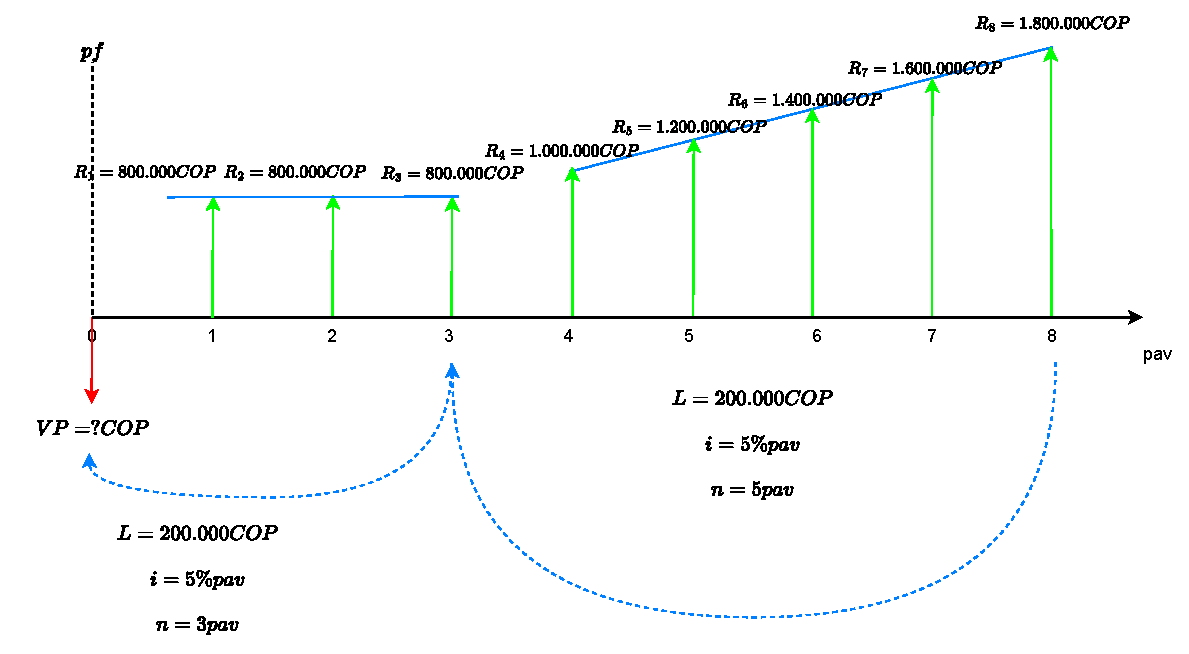
\includegraphics[trim=-5 -5 -5 -5 , scale=0.4]{6_Capitulo/ejemplos/3/Capitulo6Ejemplo3b.pdf} }

		\\ \hline
		%%%%%%%%%%%%% FIN INSERCIÓN DE IMAGEN
		%%%%%FIN FLUJO DE CAJA

		%%%%% INICIO DECLARACIÓN FORMULAS
		%%%%%%%%%%% INICIO TITULO
		\rowcolor[HTML]{FFB183}
		\multicolumn{3}{|c|}{\cellcolor[HTML]{FFB183}\textbf{4. Declaración de fórmulas}}                                                                                                                                                             \\ \hline
		%%%%%%%%%%% FIN TITULO
		%%%%%%%%%%% INICIO MATEMÁTICAS

		\multicolumn{3}{|c|}{$VP=R(\frac{1-(1+i)^{-n}}{i})+\frac{L}{i}[\frac{1-(1+i)^{-n}}{i}-n(1+i)^{-n}] \hspace{0.4 cm} \textit{Valor presente gradiente aritmético}$}                                                                             \\
		\multicolumn{3}{|c|}{$VP=R(\frac{1-(1+i)^{-n}}{i}) \hspace{0.4 cm} \textit{Valor presente de una serie unifrome vencida}$}                                                                                                                    \\
		\multicolumn{3}{|c|}{$P=F(1+i)^{-n} \hspace{0.4 cm} \textit{Valor presente dado un valor futuro}$}                                                                                                                                            \\ \hline

		%%%%%%%%%% FIN MATEMÁTICAS
		%%%%%% INICIO DESARROLLO MATEMÁTICO
		\rowcolor[HTML]{FFB183}
		%%%%%%%%%%INICIO TITULO
		\multicolumn{3}{|c|}{\cellcolor[HTML]{FFB183}\textbf{5. Desarrollo matemático}}                                                                                                                                                               \\ \hline
		%%%%%%%%%% FIN TITULO
		%%%%%%%%%% INICIO MATEMÁTICAS
		\multicolumn{3}{|c|}{$VP=  800{.}000COP(\frac{1-(1+0.05)^{-3}}{0.05})+[  1{.}000{.}000COP(\frac{1-(1+0.05)^{-5}}{0.05})+\frac{  200{.}000COP}{0.05}[\frac{1-(1+0.05)^{-5}}{0.05}-6(1+0.05)^{-6}]]$} \\
		\multicolumn{3}{|c|}{$*(1+0.05)^{-3}\hspace{0.2 cm}\textit{Ec. eqv.}$}\\
		\multicolumn{3}{|c|}{$VP= 7{.}341{.}634 \textit{  COP }$}                                                                                                                                                                                       \\ \hline


		%%%%%%%%%% FIN MATEMÁTICAS
		%%%%%% FIN DESARROLLO MATEMÁTICO
		%%%%%% INICIO RESPUESTA
		\rowcolor[HTML]{FFB183}
		%%%%%%%%%%INICIO TITULO
		\multicolumn{3}{|c|}{\cellcolor[HTML]{FFB183}\textbf{6. Respuesta}}                                                                                                                                                                           \\ \hline
		%%%%%%%%%% FIN TITULO
		%%%%%%%%%% INICIO RESPUESTA MATEMÁTICA
		\multicolumn{3}{|c|}{{$\textit{El valor presente de la serie es  7{.}341{.}634 COP }$}}
		\\ \hline
		%%%%%%%%%% FIN MATEMÁTICAS
		%%%%%% FIN RESPUESTA
	\end{longtable}
	%Se crean dos lineas en blanco para que no quede el siguiente texto tan pegado
	%\newline \newline %USARLO SI CREES QUE ES NECESARIO
\end{center}
%%%%%%%%%%%%%%%%%%%%%%%%%%FIN EJERCICIO 3.2 %%%%%%%%%%%%%%%%%%%%%%%%%%%


